\documentclass[../Main.tex]{subfiles}

\begin{document}
\author{Reflection and Refraction} %use author for title of lesson
\date{Year 1 Topic 17} %use date to refer to topic in main booklet

\section{Reflection and Refraction} %Section is the title of the lesson repeated, ready for the main contents page.

\begin{frame}{Reflection}
    When light is incident upon certain surfaces it will reflect. From intuition and experience you will know that it reflects off at the same angle it is incident upon.
    \pause
    \begin{block}{Law of reflection}
    The angle of incidence is equal to the angle of reflection.
    \begin{figure}
        \centering
        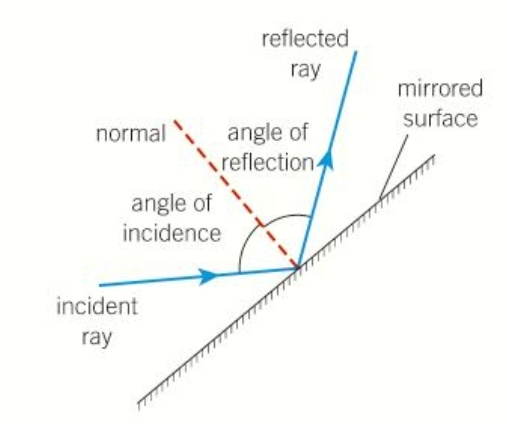
\includegraphics[width=4cm]{Waves_Images/lawofreflection.jpg}
    \end{figure}
    \end{block}
    *an exam question may ask you to draw in a light ray that is reflected! Be sure to use a ruler!
\end{frame}

\begin{frame}{Reflection}
    The most important part of the angles used is that it must be with reference to the normal to a surface. 'The normal` is an imaginary line that is perpendicular to the surface at a point. This is true even for curved surfaces. 
    
    \begin{exampleblock}{Ray diagrams}
    Complete the ray diagrams - use a ruler!!!
    \begin{figure}
        \centering
        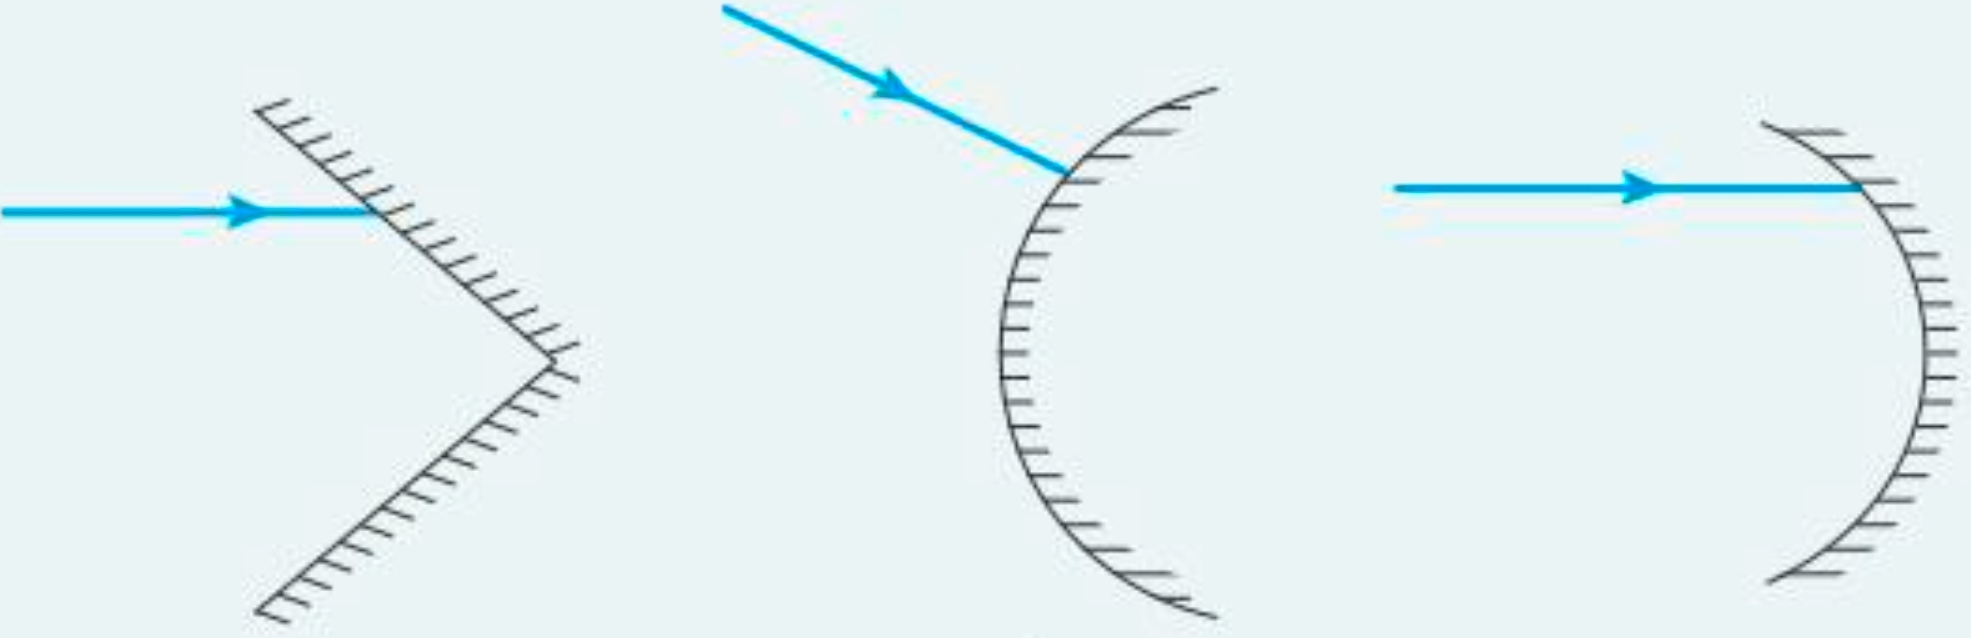
\includegraphics[width=\textwidth]{Waves_Images/raydiagrams.jpg}
    \end{figure}
    \end{exampleblock}
\end{frame}

\begin{frame}{Reflection}
    A reflected wave doesn't necessarily need to be light, and it can be represented as a series of wavefronts, each one wavelength apart. It is also true for a circular wavefront. When reflecting, the wavelength of the wave does not change, but the reflected wave is exactly $\pi$ out of phase from the original.
    \begin{figure}
    \begin{subfigure}
        \centering
        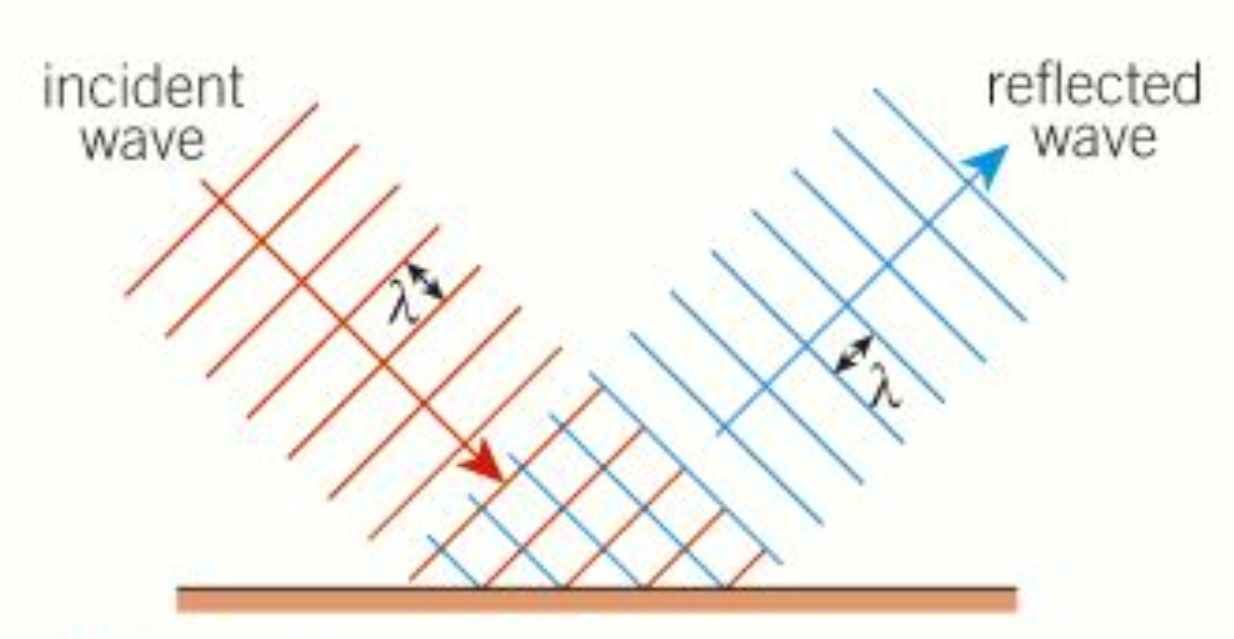
\includegraphics[height=4cm]{Waves_Images/wavefront_reflections.jpg}
        \end{subfigure}
        \begin{subfigure}
            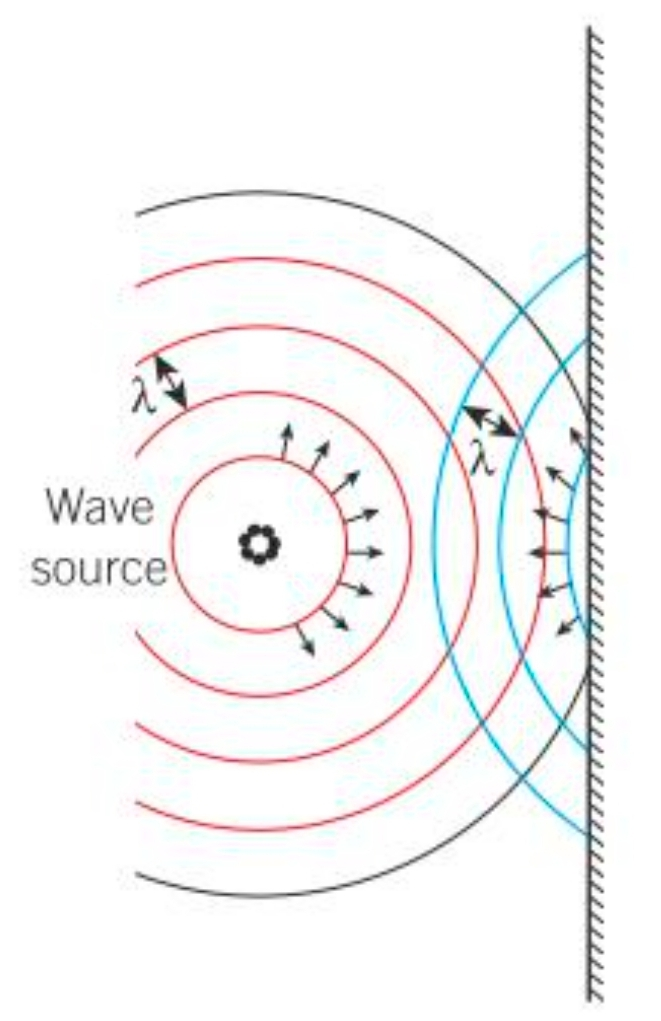
\includegraphics[height=4cm]{Waves_Images/circularwavefront.jpg}
        \end{subfigure}
    \end{figure}
    
But most exam questions will be based on light, in which case you can use a simple ray diagram.
\end{frame}

\begin{frame}{Refraction}
    When a wave enters a new medium, it will change speed. Usually this is due to resistance in the new medium.
\pause
\begin{itemize}
    \item If a wave increases speed, it will change direction, bending away from the normal line. \pause 
    \item If a wave decreases speed, it will change direction again, but bending towards the normal line.
\end{itemize}

\begin{figure}
    \centering
    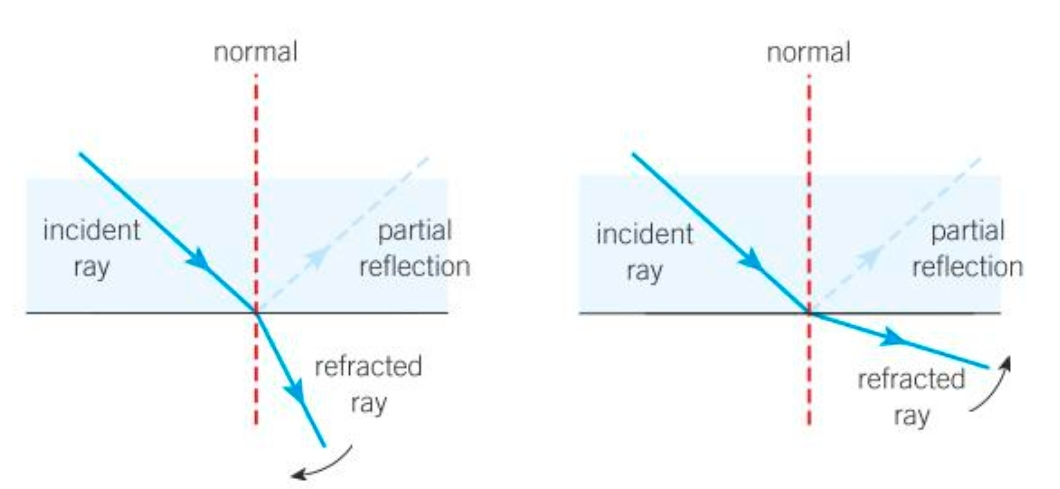
\includegraphics[height =4cm]{Waves_Images/lawofrefraction.jpg}
\end{figure}
\end{frame}

\begin{frame}{Refraction}
To know which occurs when going from one medium to another depends on the type of wave. Generally, sound, which relies on the density of the medium to affect its speed, will refract away from the normal entering a higher density medium. \pause
\begin{figure}
    \begin{subfigure}
    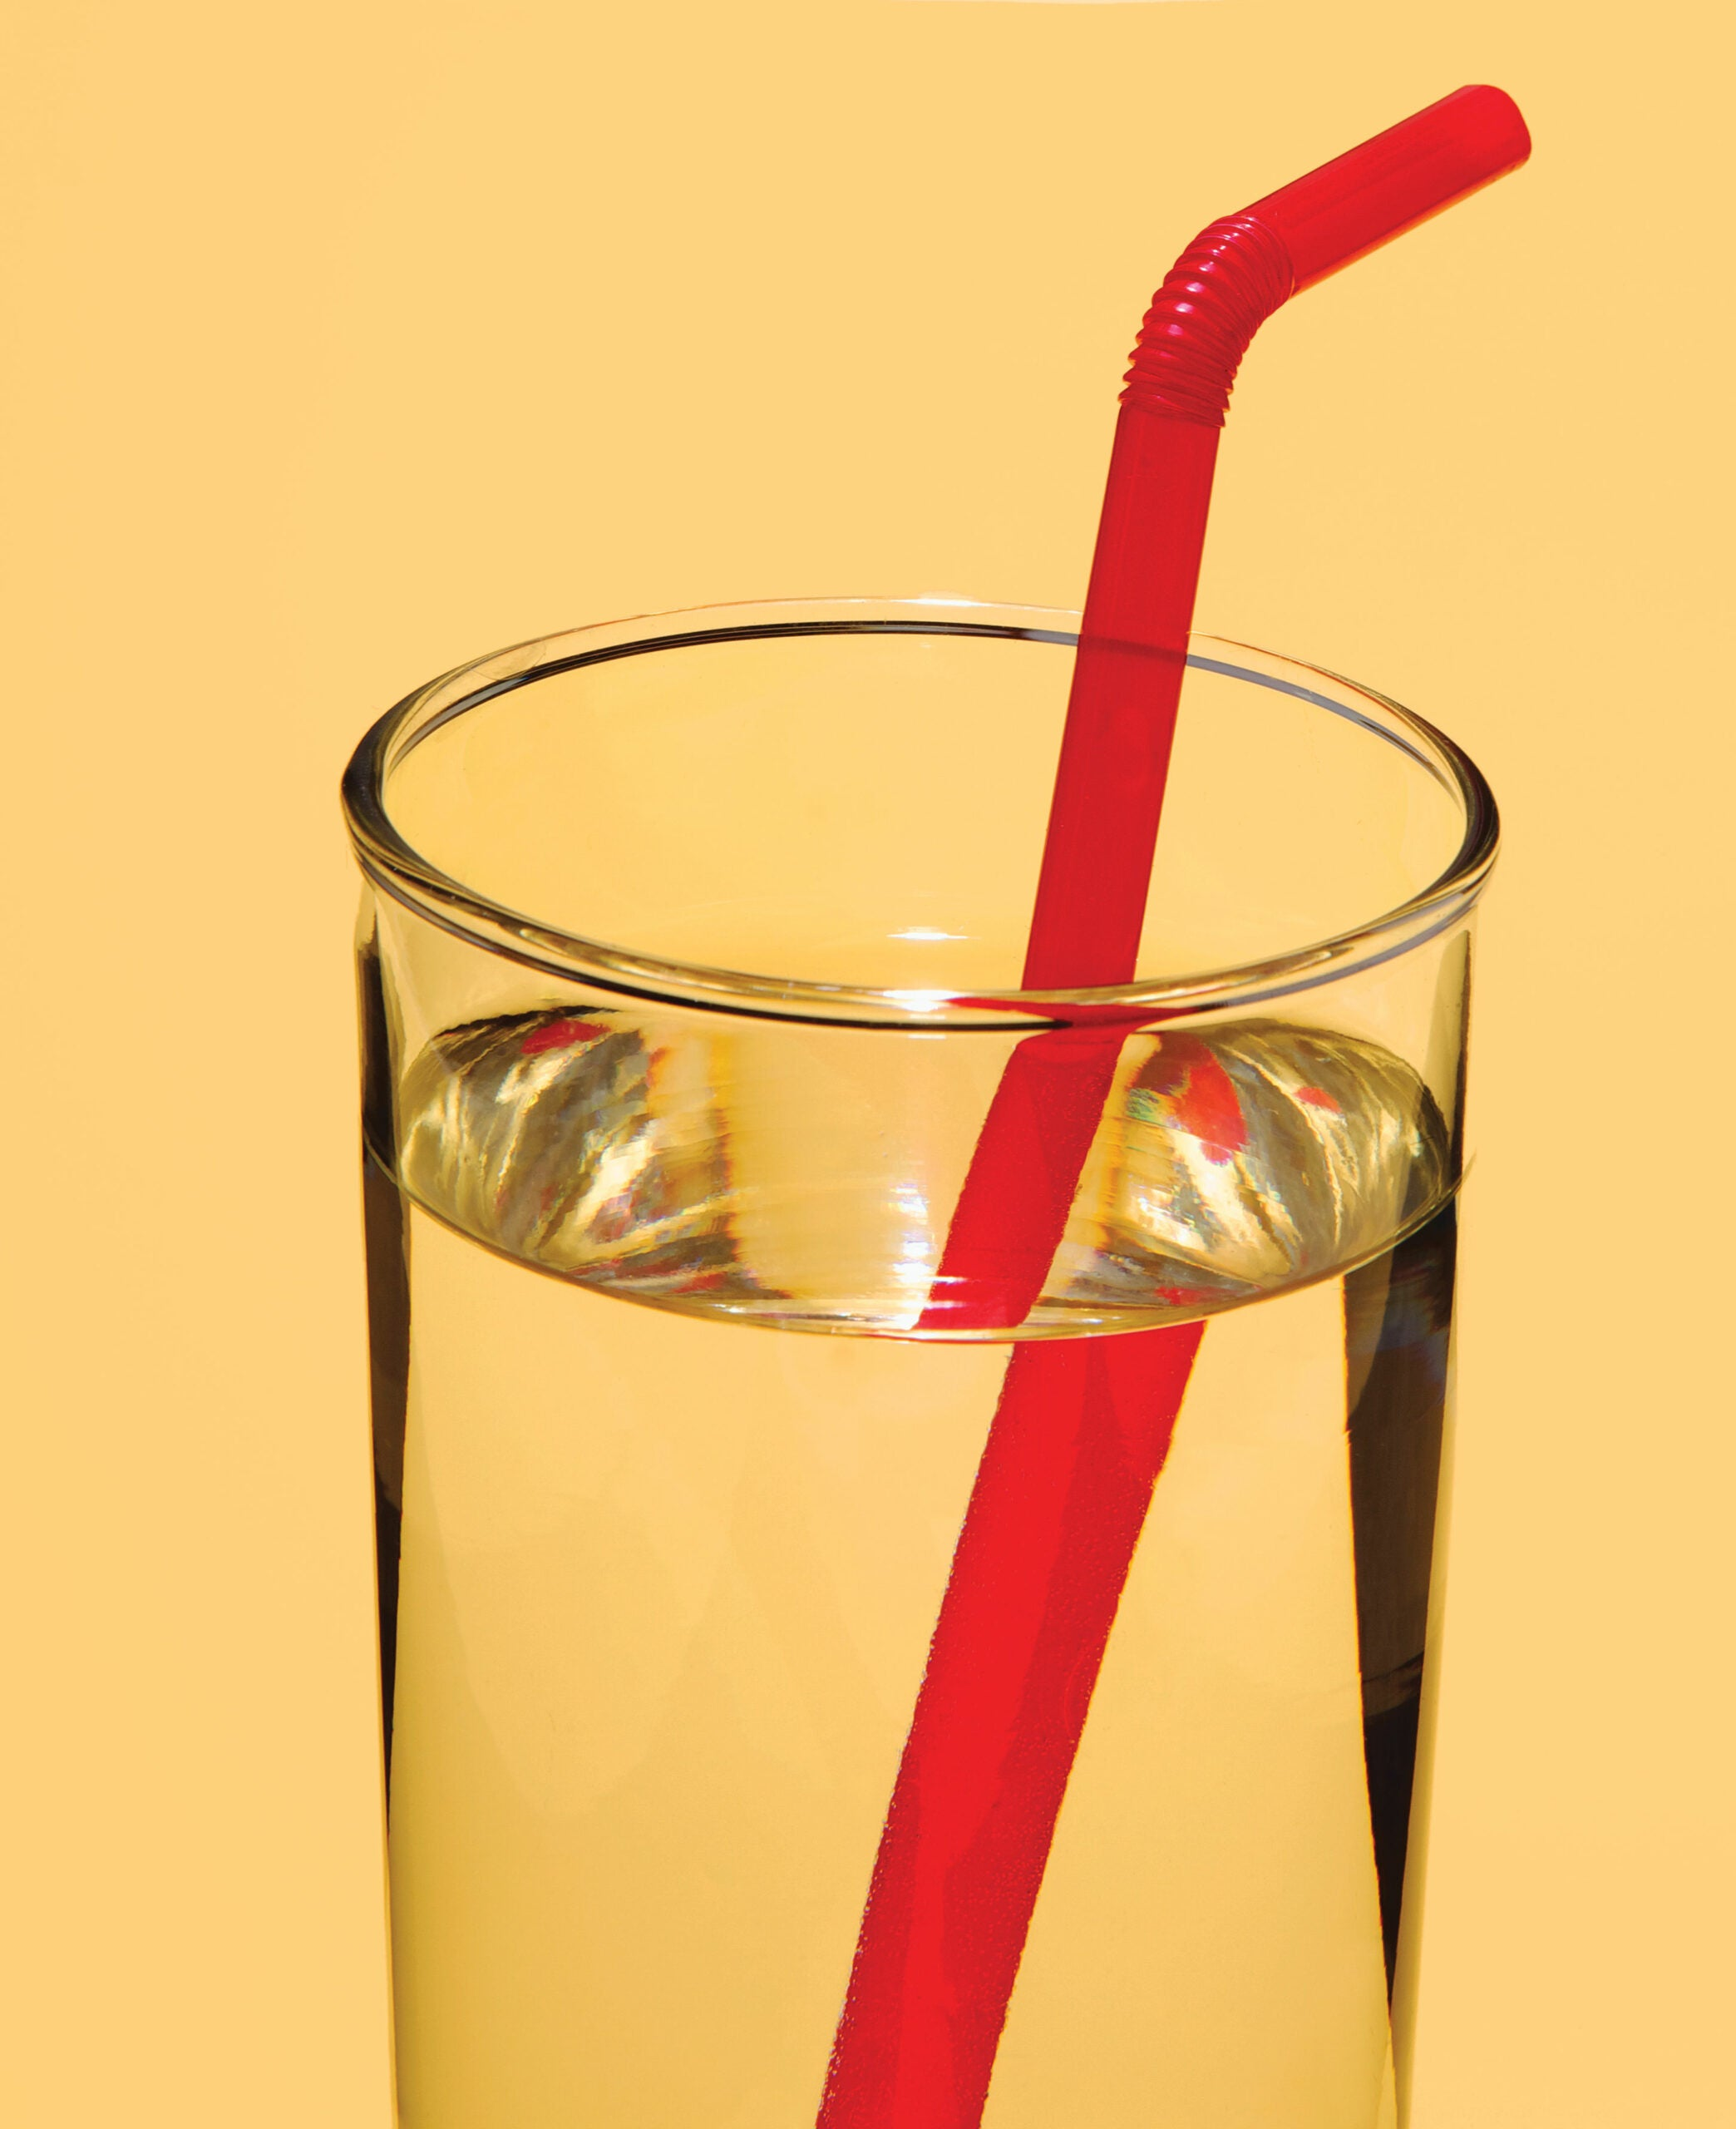
\includegraphics[height=4cm]{Waves_Images/strawbend.jpg}
    \end{subfigure}
    \begin{subfigure}
    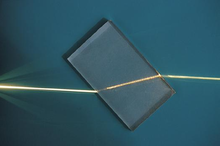
\includegraphics[height=4cm]{Waves_Images/Refraction_photo.png}
    \end{subfigure}
    \end{figure}
Whereas light, which is impeded by mediums, will bend towards the normal entering a higher density medium -- of course assuming it is transparent to light. 
\end{frame}

\begin{frame}{Refractive Index}
    Specifically for light from now on, we can introduce the concept of a refractive index. For a given medium, the higher the refractive index, the more a light ray will refract. It has no units, and is denoted with the letter 'n`.
    \pause
    \begin{alertblock}{Useful refractive indexes}
    \begin{itemize}
        \item The refractive index of a vacuum,  n=1.
        \item The refractive index of air, n=1 (actually 1.000293)
        \item The refractive index of glass, n$\approx$1.5
    \end{itemize}
    
    \end{alertblock}
\pause
    The refractive index can be calculated, and is the ratio of the speed of light in a vacuum to the speed of light in the medium.
    
    \begin{equation*}
        n=\frac{c}{v}
    \end{equation*} -- remember the speed of light in a vacuum, $c=3.00\times 10^8$ ms$^{-1}$.
\end{frame}

\begin{frame}{Refractive Index}
\begin{exampleblock}{Example}
The speed of light in water is $2.25 \times 10^8$ ms$^{-1}$. Calculate the refractive index of water. \pause
--1.33
\end{exampleblock} \pause
    \begin{exampleblock}{Example}
    The refractive index of glass is 1.4. Calculate the speed of light in glass. \pause
    \newline -- $2.1\times 10^8$ ms$^{-1}$
    \end{exampleblock}
    \begin{exampleblock}{Example}
    Calculate the speed of light in both of these materials.
    \begin{figure}
        \centering
        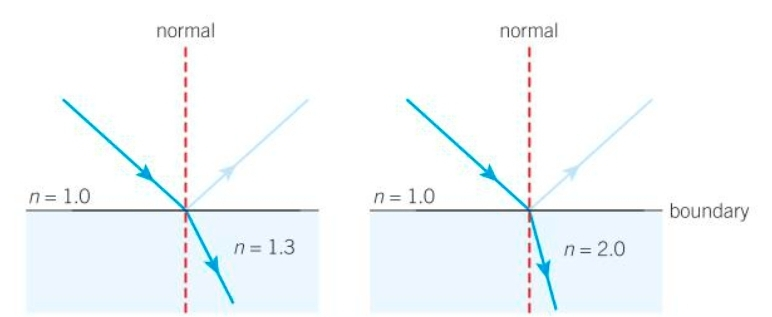
\includegraphics[height=1.5cm]{Waves_Images/refractiveindexexample.jpg}
    \end{figure} \pause
    --$2.3\times 10^8 ms^{-1}, 1.5\times 10^8 ms^{-1}$
    \end{exampleblock}
\end{frame}
\begin{frame}{Angle of refraction}
\begin{multicols}{2}
    When refracting, a light ray will move towards or away from the normal. If we take the angle of incidence to be defined similarly to before as the angle between the ray and the normal line, we can easily calculate the angle after entering/leaving a medium. 
    \columnbreak
    \begin{figure}
        \centering
        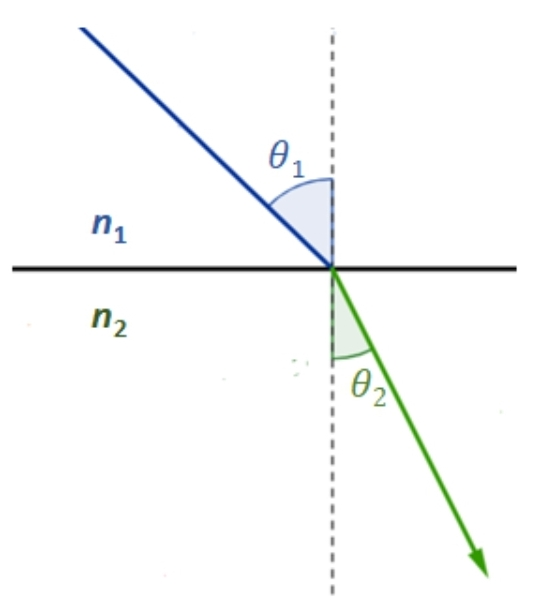
\includegraphics[height=4cm]{Waves_Images/snellslaw.jpg}
    \end{figure}
    \end{multicols}
    \begin{block}{Snell's Law}
    \begin{equation*}
        n_1 sin\theta_1 = n_2 sin \theta_2
    \end{equation*}
    On your data sheet, this is given as n$sin\theta=$constant.
    \end{block}
  \end{frame}

\begin{frame}{Snell's Law}
    \begin{exampleblock}{Example}
    Calculate the refractive index of material B.
    \begin{figure}
        \centering
        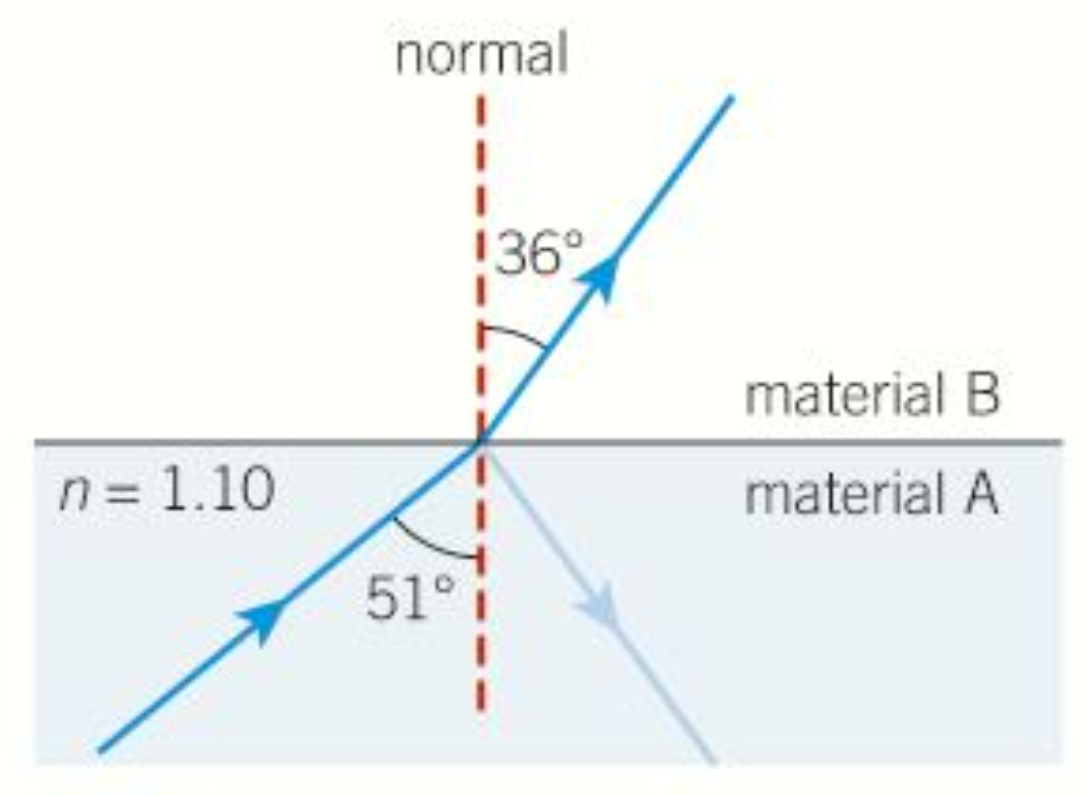
\includegraphics[height=3cm]{Waves_Images/snellslawexample.jpg}
    \end{figure} \pause
    --n=1.45
    \end{exampleblock} \pause
    \begin{exampleblock}{Example 2}
    A ray of light, travelling in air, passes into a glass block at an angle of 65° to the normal in air. The refractive index of glass is 1.5. Calculate the angle of refraction. \pause 
    -- $\theta$=37.1
    \end{exampleblock}
\end{frame}
\end{document}